\documentclass{article}
\usepackage{../fasy-hw}
\usepackage{ wasysym }
\usepackage{fancyvrb}

%% UPDATE these variables:
\renewcommand{\hwnum}{4}
\title{Advanced Algorithms, Homework \hwnum}
\author{Nathan Stouffer \and Kevin Browder}
\collab{n/a}
\date{due: 6 October 2020}

\begin{document}

\maketitle

This homework assignment should be
submitted as a single PDF file to to Gradescope.

General homework expectations:
\begin{itemize}
    \item Homework should be typeset using \LaTeX.
    \item Answers should be in complete sentences and proofread.
    \item This homework can be submitted as a group.
\end{itemize}

\nextprob
\collab{Nathan Stouffer and Kevin Browder}

You should make at least ten contributions to the Piazza board
discussing the solutions to Problems in Chapter 3 of the textbook.  Your
contribution does not have to be a complete solution.  It can be any element of
a full solution to a problem requiring an algorithm as an answer.  (For this
question, the outcomes are: insufficient posts (-1), low pass (+1), pass (+3),
and high pass (+5).

As a reminder, a full solution to a textbook problem will have the following elements:
\begin{enumerate}
    \item Describe the problem in your own words, including
        describing what the input and output is.
    \item Describe, in paragraph form, the algorithm you propose.
    \item Provide a nicely formatted algorithm to solve the problem.
    \item Use a decrementing function to prove that algorithm terminates.
    \item Give the runtime with justification.
    \item If there is a loop or recursion, what is the loop/recursion invariant? Provide the proof.
\end{enumerate}

\paragraph{Answer}

% ============================================

Our groups contributions are:
\begin{enumerate}
    \item (Chapter 3, Question 32 at 3:51 pm on October 4) \\
        Before going over a recursive idea, let's talk about some assumptions.
        First let's assume that we require 0 1's to construct 0.
        I am also going to assume that we can construct a negative number by multiplying any construction for a positive number by -1 (since the problem says we should consider any integer n as input.
        Then since we can give the answer for any negative integer -n by computing 1 + the answer for n and we know the answer for n=0 to be 0, let's assume that our input is preprocessed as follows:

        \begin{algorithm}
            minN(n): \\
            $\cdot$ \hspace{1.5em} if (n == 0): return 0 \\
            $\cdot$ \hspace{1.5em} else if (n $>$ 0): return 1 + minNrec("(1)", n) // add one because we seed a 1 in the input expression \\
            $\cdot$ \hspace{1.5em} else: return 1 + 1 + minNrec("(1)", abs(n)) // n must be negative so add the extra 1
        \end{algorithm}

        Then we can give the description for minNrec(expr, n) with the assumption that we have input starting with the expression string (1) and are trying to obtain a natural number n.
        In English, we should perform the following steps.
        First, test if expr evaluates to n.
        If so, return 0. If expr evaluates to larger than n, return +inf. Otherwise, we should test each path from the current expression (this would be adding 1 inside the parenthesis, adding one outside the parenthesis, and multiplying by (1 + 1).
        Then we can take the minimum of the returned values (as long as we add the how many ones are used in each pathway, see the psuedocode for an explicit example of what I mean).

        To be more explicit about the three choices.
        Adding an internal one would be like taking (1+1)*(1+1) to (1+1)*(1+1+1).
        Adding an external on would be like taking (1+1)*(1+1) to (1+1)*(1+1) + (1).
        Multiplying by (1+1) would be like taking (1+1)*(1+1)*(1+1).
        The reason we multiply by (1+1)=2 instead of by (1) is because multiplying by (1) would result in some branches of the recursion tree never terminating (always multiplying by 1).

        As a mathematical formula, I am not really sure what you mean by this.
        The way I thought about it, we are really just adding a bunch of ones up.
        I think the psuedocode gives the best example of the mathematical formula.

        So here is the psuedocode.
        Note that expr is a string so we take + to be concatenation.
        Also note that evaluate() takes in an expression string and computes the integer that it evaluates to.

        \begin{algorithm}
            minNrec(expr, n) \\
            $\cdot$ \hspace{1.5em} if (evaluate(expr) == n): return 0 \\
            $\cdot$ \hspace{1.5em} else if (evaluate(expr) $>$ n): return +inf \\
            $\cdot$ \hspace{1.5em} add\_internal\_one = 1 + minNrec(expr[:len(expr)-1] + "+1)", n) \\
            $\cdot$ \hspace{1.5em} add\_external\_one = 1 + minNrec(expr + "+(1)", n) \\
            $\cdot$ \hspace{1.5em} mult\_by\_two = 1 + 1 + minNrec(expr + "*(1+1)", n) \\
            $\cdot$ \hspace{1.5em} return min \{ add\_internal\_one, add\_external\_one, mult\_by\_two \}
        \end{algorithm}
    \item (Chapter 3, Question 46 at 4:10 pm on October 4) \\
        The problem we would like to solve needs two things: the hierarchy of the Giggle company and how much ``fun'' each employee is.
        The goal is to create a guest list of employees that results in the maximum amount of fun had at the party.
        To compute the amount of fun at the party, we get the fun value of each employee on the guest list and compute the sum of all those fun values.
        However, we cannot just greedily select all the employees with positive fun values to attend the party.
        We must include the president of the company.
        Additionally, putting an employee on the guest list means that their immediate underlings cannot attend the party.
        Subject to these constraints, we would like for the employees to have the most fun possible.
    \item (Chapter 3, Question 46 at 10:00 am on October 4) \\
        Here is a more precise description of the problem. As Brittany said, let Giggle have $n$ employees and ids that range from 1 to $n$ (we include the president in this list and the president has employee id 1). Then we have the level of fun that each employee brings to the party, labeled as $fun_i$ where $i$ is employee id (note that $fun_1 < 0$ but there are no other constraints on the amount of fun that other employees can bring.

        Our input should then consist of two things. First, we should have a directed graph $T$ where the vertices are the $n$ employees of the company and edges are drawn between a supervisor and their immediate underlings. The supervisor is the tail of the edge and the immediate inferior is the tip of the edge. $T$ is necessarily a tree, otherwise there would be some weird power relationships in the company. The second part of our input should be an array where the $i^{th}$ entry contains $fun_i$. This way, we can access the level of fun that each employee brings.

        The algorithm will return a set of natural numbers $A$ (representing employee ids) such that $ \{ 1 \} \subset A \subset \{ 1, 2, ... , n \} $ and subject to the following constraint: it must be the case that if $ a \in A $, it must be true that any direct children of $a$ (with respect to the $T$) are not in $A$. With respect to the constraints of the problem, we want to return the maximum $\sum_{i \in A} fun_i $ for the company party.
    \item (Chapter 3, Question 3 at 10:20 am on October 4) \\
        In response to the runtime question that Brittany asked, we want to know whether Greg's algorithm runs in $O (n)$ time or $\Theta (n)$ time.
        The algorithm runs in $\Theta (n)$ time.
        Greg has already noted that the algorithm runs in $O (n) $ time so we only need to show that the algorithm runs in $\Theta (n) $.
        With the exception of line 4, all lines in the pseudocode run in constant time (they are all if statements, array access, ... ).
        Then line 4 runs exactly $n$ times (since the length of the array $A$ is $n$.
        So the algorithm runs in $\Theta (n)$ time.

        As for the loop invariant, the value in largest\_subarray\_sum is always $\max _{j \leq k} \sum _{l=j}^k A[l] $ such that $k \leq i$.
        In words, this is the maximum sum of contiguous values in the array such that the contiguous section appears no later than the $i^{th}$ index.
        Once the loop terminates, we will have $\max _{j \leq k} \sum _{l=j}^k A[l] $ such that $k \leq n $, which is the desired solution.
    \item (Chapter 3, Question 13 at 10:50 am on October 4) \\
        I was thinking of using the following recursive solution. In words, we want to compute the total score for each valid sequence of songs that we will dance to and return the maximum. Recall that we have Score[1..n] and Wait[1..n].

        \begin{algorithm}
            \textsc{MaxScore}(Score[1..n], Wait[1..n]) \\
            $\cdot $ \hspace{1em} if (len(Score) == 0) \hspace{9em} // test if we are at the bottom of the recursion tree \\
            $\cdot $ \hspace{2em} return 0 \\
            $\cdot $ \hspace{1em} sit = MaxScore(Score[2:], Wait[2:]) \hspace{2em} // don't dance to this one, call on remaining songs \\
            $\cdot $ \hspace{1em} w = Wait[1] \hspace{12em} // how many songs we have to wait if we dance \\
            $\cdot $ \hspace{1em} dance = Score[1] + MaxScore(Score[2+w:], Wait[2+w:]) \hspace{0.25em} // dance to this one, call on remaining songs \\
            $\cdot $ \hspace{1em} return max(sit, dance)
        \end{algorithm}
    \item (Chapter 3, Question 3b at 4:30 pm on October 4) \\
        There has been a lot of discussion on Chapter 3, Question 3a. Part b also seems pretty interesting. Here is the question:

        Suppose you are given an array $A[1..n]$ of numbers, which may be positive, negative, or zero, and which are not necessarily integers.
        Describe and analyze an algorithm that finds the largest product of elements in a contiguous array $A[i..j]$.
    \item (Chapter 3, Question 3b at 5:50 pm pm on October 4) \\
        Here is the psuedocode for what I am thinking. When I posted this, I was struggling to think about how negatives could change things up from Question 3a. But I think that there is actually no change. We can just use the following pseudocode:

        \begin{algorithm}
            MaxProd(A[1..n], i, j) \\
            $\cdot$ \hspace{1em} if ($i > j$) \\
            $\cdot$ \hspace{2em} return 1 \\
            $\cdot$ \hspace{1em} current = product(A, i, j) \\
            $\cdot$ \hspace{1em} left    = MaxProd(A, i+1, j) \\
            $\cdot$ \hspace{1em} right   = MaxProd(A, i, j-1) \\
            $\cdot$ \hspace{1em} return max(current, left, prod)
        \end{algorithm}

        This is correct because we compute the product of every subset of A and choosing the max (this seems to be a modified version of the solutions suggested so far). I agree with the analysis that this will take $O (2^n)$ time because that is the number of options that must be processed.

        Additionally, the recurrence relation for this is algorithm is $T(n) = n + 2T(n-1)$. We must add $n$ because we are multiplying $n$ things and then the $2T(n-1)$ appears because of the calls to MaxProd with arrays of length $n-1$. This recurrence relation definitely has at least an exponential bound because the 2 in the expression $T(n) = n + 2(n-1+2(n-2+2(n-3 + 2(\cdot \cdot \cdot))))$ appears $n-1$ times and simplifying it will give $2^{n-1}$.

        Conveniently, we can make a dynamic programming algorithm out of this. If $i$ indexes the rows and $j$ indexes the columns of a matrix $T$ (where $i \leq j$), then we can compute $T(i, j)$ as long as we know $T(i+1, j)$ and $T(i, j-1)$ and are willing to put in some work multiplying all the elements from $i..j$ (inclusive). Then we can just fill out the matrix computing the diagonal (since $T(i, i)$ is just $max (0, A[i])$) and then going diagonally down from $A[i, j+1]$ (and repeating this process until the top right corner is reached). Hopefully that explanation of dependencies is clear without a table/dependency graph.

        I am not sure if this is the optimal dp solution because there is that expensive linear product that must run for each entry in the table. We can at least give an upper bound for this. Filling out an entry in the table will take $O (n) + O(1) + O(1)$ time. The constant operations come from accessing the table and the $O(n)$ operation is the product of elements $i..j$. The number of entries that we must fill out in the table is the sum $\Sigma _{k=1}^n k = n(n+1)/2$ (sum found by counting from bottom right of the matrix) so this dp solution runs in $n(n+1)/2 O (n) = O(n^3)$ time. This is definitely better than exponential but I doubt that it is optimal.
   	\item (Chapter 3, Question 12 at 9:51 pm on October 6)\\
        	subproblem c: Five years later, thirteen-year-old Elmo has become a much stronger player. Describe and analyze an algorithm to determine, given the initial sequence of cards, the maximum number of points that you can collect playing against a perfect opponent.
    \begin{Verbatim}
    def elmoMax(mem, cards, myTurn):
    max = 0
    if (not cards):
        return 0
    if str(cards) in mem: #reference previously calculated state
        return mem[str(cards)]
    elif not myTurn: #Elmo's turn
        if cards[0] > cards[len(cards) - 1]:
            max = elmoMax(mem, cards[1:], True)
        else:
            max = elmoMax(mem, cards[:-1], True)
    else: #your turn
        left = cards[0] + elmoMax(mem, cards[1:], False)
        right = cards[len(cards) - 1] + elmoMax(mem, cards[:-1], False)
        max = max(left, right)
        mem[str(cards)] = max #store state
    return max
    \end{Verbatim}
    \item (HW 4 Question About Parts 1 & 2 at 9:33 pm on October 6) \\
        Question: So part one is having us 	contribute one of the six parts of a solution to a question on Piazza and part 2 is requiring us to go through all six steps, right? Are we allowed to use the answers from 4-2 in 4-1 Piazza posts? \\
        Yes, the question just says to answer in your own words for part two. You just can't copy paste other students answers into your solution.
  	\item (Chapter 3, Question 25 (Largest Rectangular SubArray Sum) at 2:00pm on October 6) \\
        Seth,

        This is a very interesting problem and I think your solution would work but it looks very expensive, $O(n^4)$ I think. I think you can apply Kadane’s algorithm which finds the longest increasing sub sequence for a one dimensional array to reduce the time complexity to $O(n^3)$. If we find top and bottom row numbers for every fixed left and right column pair. To find the top and bottom row numbers, calculate sum of elements in every row from left to right and store these sums in an array. So the indices in this array indicate sum of elements from left to right in the corresponding row If we apply Kadane’s algorithm on this array we get the maximum sum subarray of array, this maximum sum would be the maximum possible sum with left and right as boundary columns. To get the overall maximum sum, we compare this sum with the maximum sum so far.

\end{enumerate}

% ============================================

\nextprob
\collab{Nathan Stouffer and Kevin Browder}

Choose one of the Chapter 3 problems discussed in Piazza and provide a solution
in your own words.  This should be a polished solution.

\paragraph{Answer}
% ============================================

For our polished solution, we chose Chapter 3 Problem 3.
Here is the problem from the textbook.

Suppose you are given an array $A[1 .. n]$ of numbers, which may be positive, negative, or zero, and which are not necessarily integers. \\
(a) Describe and analyze an algorithm that finds the largest sum of elements in a contiguous subarray $A[i .. j]$. \\
(b) Describe and analyze an algorithm that finds the largest product of elements in a contiguous subarray $A[i .. j]$.

\begin{enumerate}
    \item First we describe the problem in our own words.
        Given an array of real numbers $A[1..n]$ with length $n$, our task is to find the maximum sum (or product) that a contiguous portion of $A$ gives.
        The minimum such value that can be returned for sums is 0 (since we take a contiguous section of length 0 to obatin this).
        Similarly, the minimum value that can be returned for the product is 1.
        We assume that the functions sum($\cdot$) and product($\cdot$) are built in an return the following values: sum($A$, $i$, $j$) $ = \Sigma _{k=i}^j A[k] $ and product($A$, $i$, $j$) $ = \Pi _{k=i}^j A[k] $ when $i \leq j$.
    \item The solutions to each of these problems are quite similar.
        At a high level, what we want to do is compute the sum/product of each contiguous subarry in $A$ and return the maximum that we find.
        The way that we do this sets us up nicely for a dynamic programming solution.
        Say we want to know the \textsc{MaxSum} starting with the index 1 and ending with index $n$.
        Let's call a function \textsc{MaxSum}($A$, $1$, $n$) that performs the following.
        First it computes the sum of the contiguous values found at indices $1..n$.
        Then it recursively calls \textsc{MaxSum} on the subarrays $A[2..n]$ and $A[1..n-1]$.
        When the recursion terminates, we return the maximum of returned values compared with sum of the entire array.
        A similar argument exists for \textsc{MaxProd} that uses the product method instead of the sum.
    \item Here is the psuedo code for our \textsc{MaxSum}.
        A slightly modified version of \textsc{MaxSum} can be used for \textsc{MaxProd}.
        \begin{algorithm}
            \textsc{MaxSum}($A[1..n]$, $i$ , $j$) \\
            1. \hspace{1em} if ($i > j$) \\
            2. \hspace{2em}     return 0 \\
            3. \hspace{1em} current = sum($A$, $i$, $j$) \\
            4. \hspace{1em} left = \textsc{MaxSum}($A$, $i+1$, $j$) \\
            5. \hspace{1em} right = \textsc{MaxSum}($A$, $i$, $j-1$) \\
            6. \hspace{1em} return max(current, left, right)
        \end{algorithm}
        \begin{algorithm}
            \textsc{MaxProd}($A[1..n]$, $i$ , $j$) \\
            1. \hspace{1em} if ($i > j$) \\
            2. \hspace{2em}     return 1 \\
            3. \hspace{1em} current = product($A$, $i$, $j$) \\
            4. \hspace{1em} left = \textsc{MaxProd}($A$, $i+1$, $j$) \\
            5. \hspace{1em} right = \textsc{MaxProd}($A$, $i$, $j-1$) \\
            6. \hspace{1em} return max(current, left, right)
        \end{algorithm}
    \item The pseudocode for the above algorithms are almost identical.
        There are only two differences, first we return a different minimum value (0 vs 1).
        Second, in \textsc{MaxSum} we sum the values $i..j$ whereas in \textsc{MaxProd} we multiply the same values.
        When each of the sum and product function are called, we know that $i \leq j$ so $0 \leq j-i$.
        We also know that $j-i \leq n$ so each function will run in $O (n)$ time (it is performing nor more than $n$ operations).

        Other than those two small differences, the algorithms are identical in structure.
        So if we prove termination and partial corretness one of them, the same must be true for the other.
        From here on, we will only focus on \textsc{MaxSum}, but our results apply to \textsc{MaxProd} as well.

        So we must now show termination for \textsc{MaxSum}.
        Certainly lines 1 and 2 will terminate since they run in constant time.
        Line 3 runs in $O(n)$ time (shown above), so it will terminate.
        Additionally line 6 will terminate because max runs in linear time.
        So we now need only show that lines 4 and 5 terminate.
        We do so with a decrementing function.

        Let our state space be the length of the array that is being considered in a recursive call $R_i$.
        This is the contiguous range of values $i..j$ (inclusive).
        This maps to the natural number $j-i+1$ (adding 1 because the bounds are inclusive).
        The left recursive call $R_{i+1}^l$ considers the contiguous range $i+1..j$ which maps to the natural number $j-(i+1)-1 = j-i$ which is strictly less than $j-i+1$.
        So the left recursive call must terminate.
        Similarly, the right recursive call $R_{i+1}^r$ considers the contiguous range $i..j-1$ which maps to the natural number $j+1-i+1 = j-i$ which is strictly less than $j-i+1$.
        Therefore, the right recursive call must terminate.

        Since every line in the \textsc{MaxSum} algorithm terminates, the entire algorithm must terminate.
    \item We must now show partial correctness under the assumption that the algorithm terminates.
        Our invariant is that the left and right recursive calls always contain the maximum sum in their respective ranges.
        This is certainly true in the base case of $i > j$ since $i > j$ does not reference a contiguous portion of the array so all we can do is return that the maximum sum is 0.
        Towards induction, now suppose that, for some $i,j$ such that $i \leq j$, we have the fact that the left and right recursive calls each contain the maximum sum of contiguous values in their respective ranges.
        We then have three things: the sum stored in current ($max_c$), the maximum sum in the range $i+1..j$ ($max_l$), and the maximum sum in the range $i..j-1$ ($max_r$).
        If $max_c$ is larger than both $max_l$ and $max_r$ then $max_c$ is the largest sum in the range $i..j$.
        However, if one of $max_r, max_l$ is larger, then $max_c$ cannot be the maximum sum in $i..j$.
        So we should return the max of the current, left, and right gives the maximum sum in $i..j$.
        This proves the inductive step, implying that the invariant is true at all points in the recursion tree.
        Since we already know that the algorithm terminates and it follows that the algorithm will terminate in some branch of the recursion tree, it must terminate in a correct state.
        Thus our algorithm is correct.
    \item So we have proven that the above algorithms produce correct solutions of the contiguous sum/product problem.
        However, they are quite slow.
        Conveniently, we can make a dynamic programming algorithm out of our current solutions.
        If $i$ indexes the rows and $j$ indexes the columns of a matrix $T$ (where $i \leq j$), then we can compute $T(i, j)$ as long as we know $T(i+1, j)$ and $T(i, j-1)$ and are willing to put in some work add all the elements from $i..j$ (inclusive).
        Then we can just fill out the matrix by computing the diagonal (since $T(i, i)$ is just $max (0, A[i])$) and then going diagonally down from $A[i, j+1]$ (and repeating this process until the top right corner is reached).
        Here is a drawing of the matrix for the case of $n=5$:
        \newpage
        \begin{figure}
            \begin{center}
                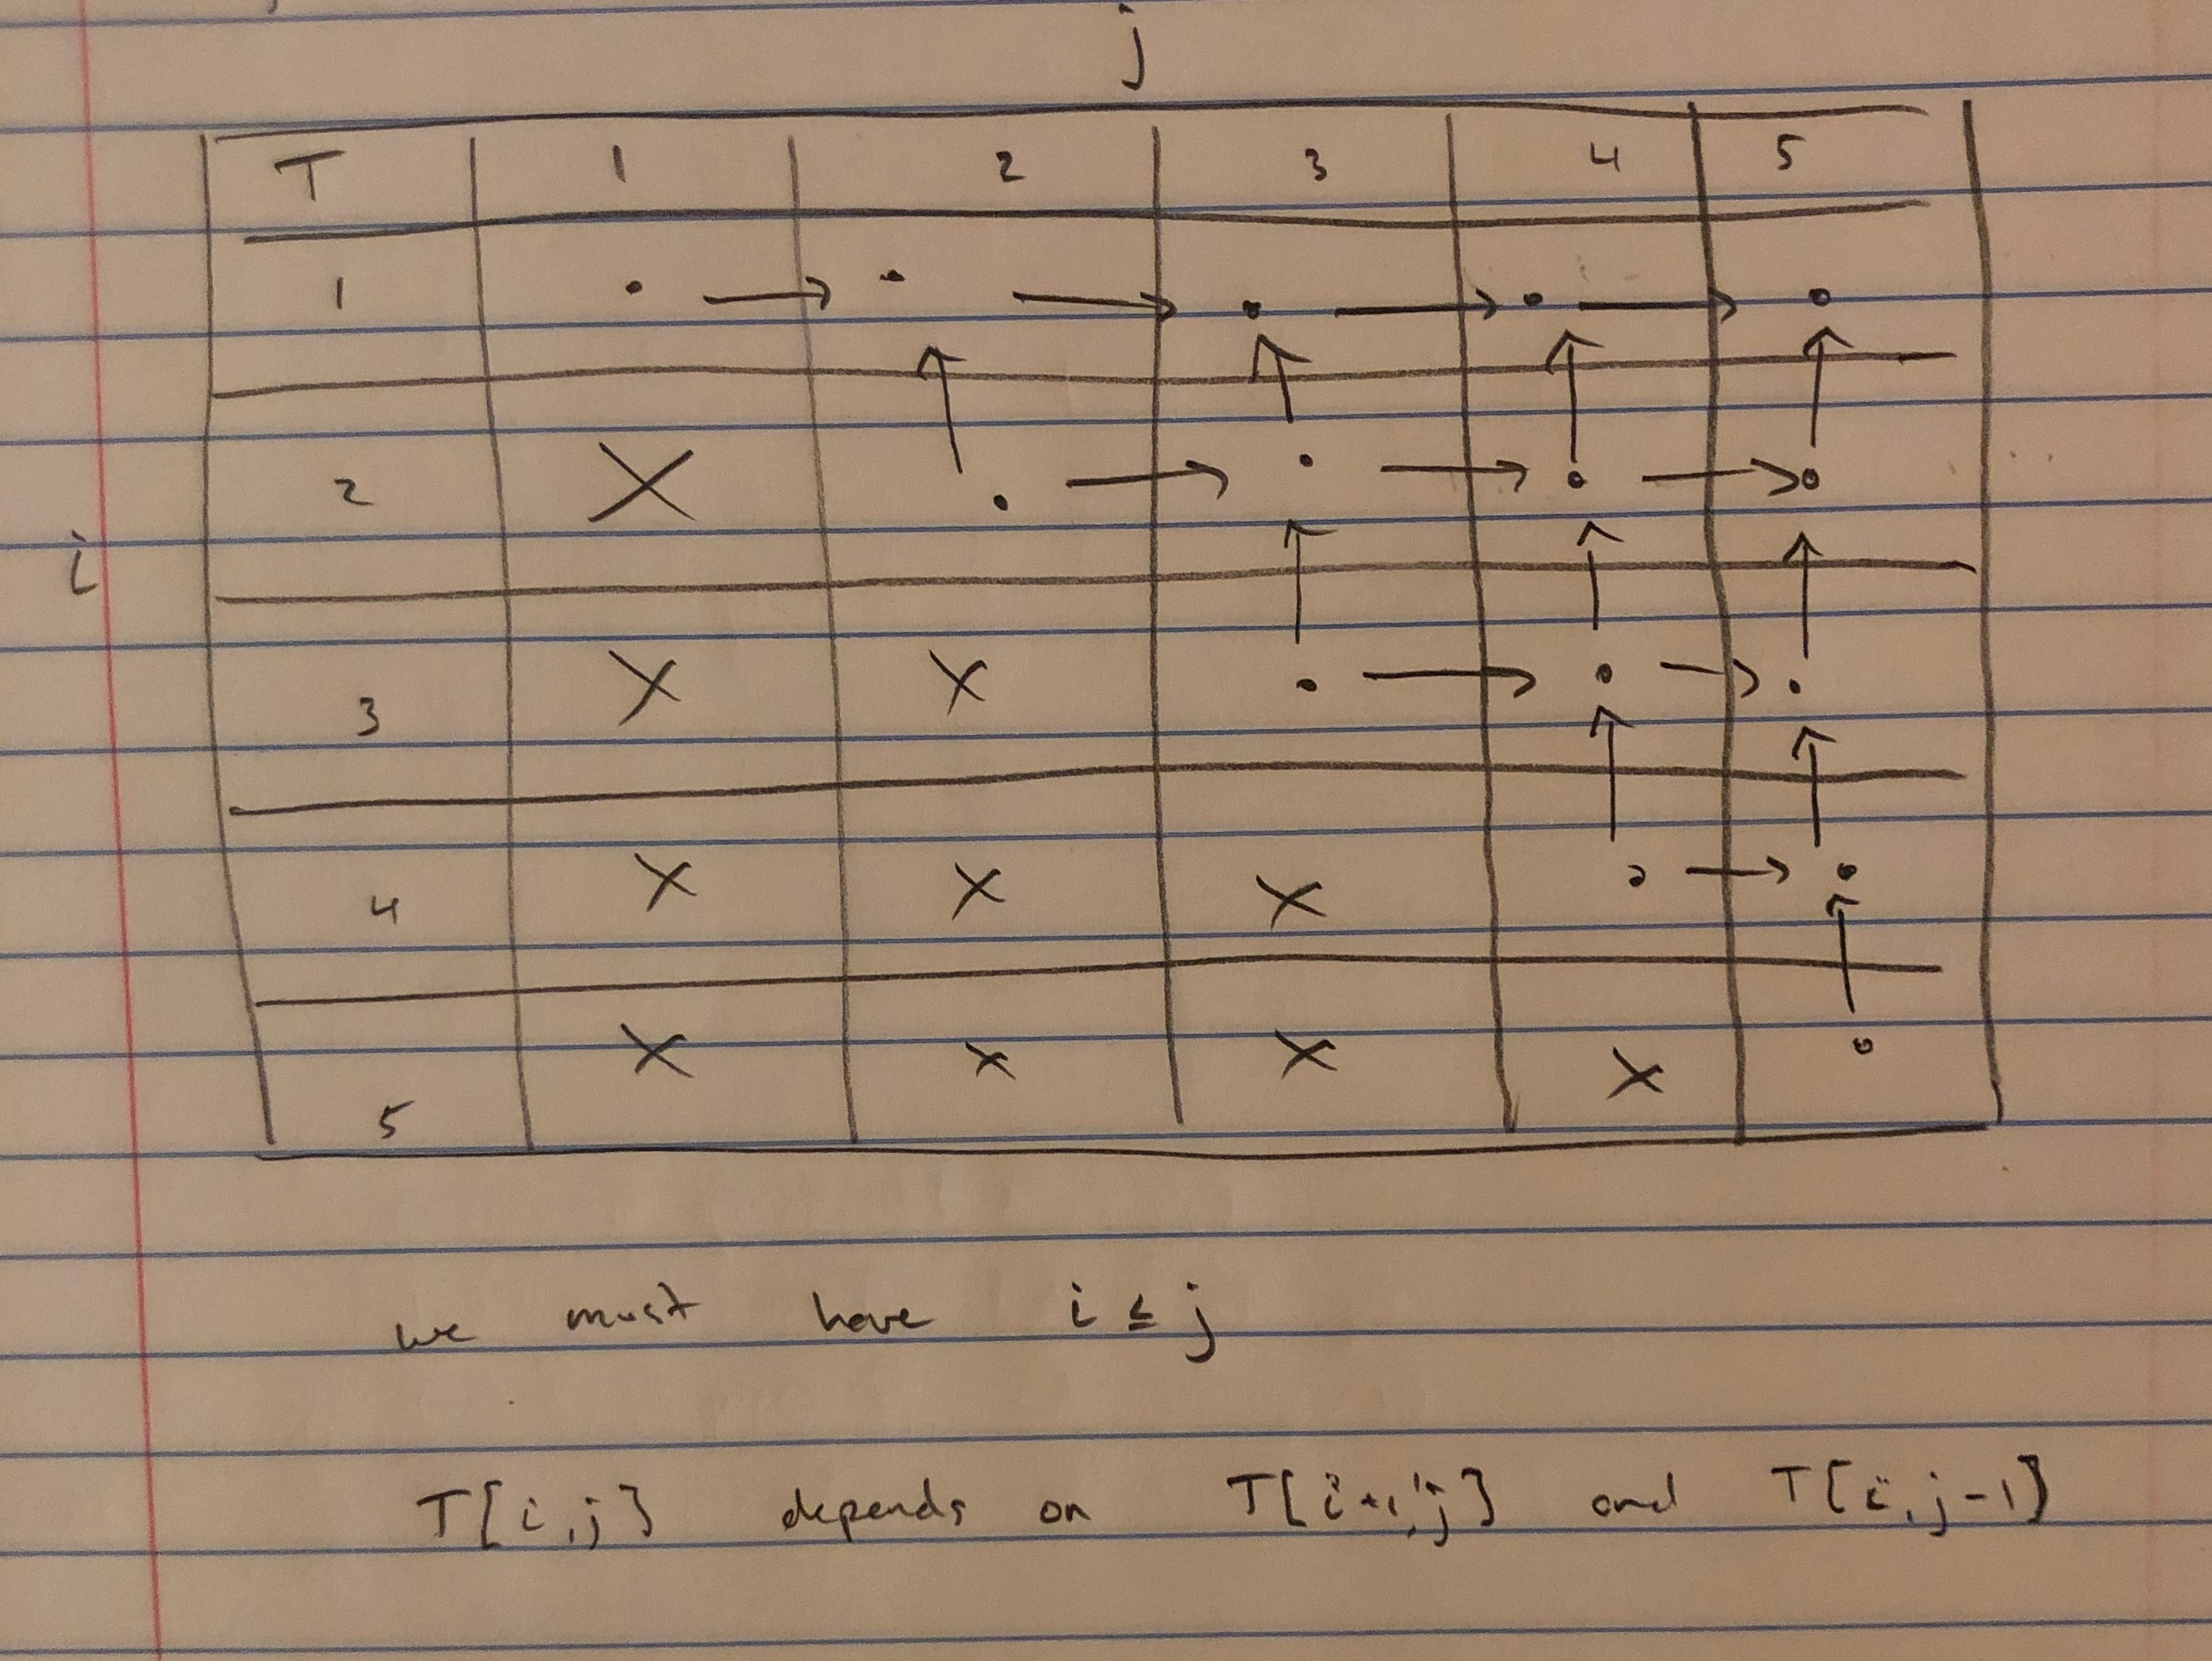
\includegraphics[scale=0.1]{image0}
                \caption{Dependency Table for $n=5$}
    		    \label{fig:dynprog}
            \end{center}
        \end{figure}

        We are not sure if this is the optimal dynamic programming solution because there is that expensive linear sum that must run for each entry in the table.
        But we can at least give an upper bound for how long our new dynamic programming solution takes.
        Filling out an entry in the table will take $O (n) + O(1) + O(1)$ time.
        The constant operations come from accessing the table and the $O(n)$ operation bounds time taken to sum of the elements found from $i$ to $j$.
        The number of entries that we must fill out in the table is the sum $\Sigma _{k=1}^n k = n(n+1)/2$ (sum found by counting from the bottom right of the matrix) so this dynamic programming solution runs in $(n(n+1)/2) * O (n) = O(n^3)$ time.
\end{enumerate}

% ============================================

\nextprob
\collab{Nathan Stouffer and Kevin Browder}

For this problem, choose either the Edit distance algorithm (Section 3.7) or the
Subset Sum problem (Section 3.8). Look at three different sources (including the
textbook) that describe
and analyze the same algorithm. In one to two pages, describe the similarities
and differences in the presentation and analysis of the algorithms.

\paragraph{Answer}

% ============================================

	We choose to look at the Edit Distance Algorithm from Section 3.7 of the textbook. Our three sources were the textbook, GeeksforGeeks\footnote{Edit Distance: DP-5, GeeksforGeeks, January 13, 2020, https://www.geeksforgeeks.org/edit-distance-dp-5/.} and a Stanford lecture\footnote{Dan Jurafsky, “Minimum Edit Distance,” Stanford University, n.d., https://web.stanford.edu/class/cs124/lec/med.pdf.}. All  three presentations begin with a quick definition of the what the algorithm actually does in words. The textbook goes into much more detail than the other two sources but all sources include a quick example showing the algorithm working and the resulting output. Stanford's presentation also touches on practical implementation of Edit distance including spell check, computational biology and others. After this introduction GeeksforGeeks and the textbook dive into the subproblems and recursive approach to this problem. The Stanford article touches on the naive approach briefly but not in the depth that the other two look at it. GeeksforGeeks gives fully functional code in 5 languages for the naive approach while the textbook just describes it. All three sources go over the downsides of recursion because you have to cover a lot of possibilities multiple times and the resulting exponential time complexity.\\
	 All three sources then go into dynamic programming as the solution to this issue. GeeksforGeeks is the most code oriented source. After they briefly go over the time complexity issue with the naive recursive solution they dive right into the dynamic programming source code in 5 languages again complete with sample input and output and time complexity. They provide two separate solutions with the second being more optimized for space complexity as the first solution becomes unusable when the string lengths are greater than 2000. They then give a short video that gives an overview of everything I have described. I personally really liked their write up and it is very practically oriented.  \\
	 Stanford goes in another direction, they give some pretty high level pseudo code and then dive into an example edit distance table and go over how it is filled up with an example. They also give the completed table. They then add backtracing to the table and walk through the pseudo code for that as well. They also give the time complexity for each step. They then give the distance matrix. They then go on to some more complicated topics like weighted edit distance and applying this concept to sequence alignment in the form of natural language processing and computational biology. I did really enjoy how they included real life examples outside of academics but their deep dive into the tables was not very helpful and I through it added more confusion than clarification. That also might be because it is power point that is meant to be a lecture.\\
	The textbook kind of combines the previous two sources. They give a lot more setup for the dynamic programming solution including subproblems, memoization struture, dependencies, evaluation order and space and time. They also give some very nice pseudo code that is much better than the other two sources. They also give a memoization table that is much nicer and easier to read than the Stanford one. It is also just the completed table which takes a lot less room. The only think I do not like about the textbook writeup is that they don't give any sort of context or idea of where you would apply this algorithm which I really like. Other than than I think this source does the best job of explaining the algorithm.
% ============================================

\end{document}
